% Giles (2000) has a good discussion on this.
% \cite{ma_comparison_2021}. 

In this section, we are going to address how these different methods are computationally implemented and how to decide which method to use depending on the scientific task.
In order to address this point, it is important to make one more further distinction of the methods introduced in Section \ref{section:methods} between those that apply direct differentiation at algorithmic level or those that are based on numerical solvers.  
The first are easier to implement since their are agnostic with respect to the details of the ODE and its numerical solution; however, they tend to be either inaccurate, memory expensive, or unfeasible for large models. 
The family of methods that are based on numerical solvers include the sensitivity equations and the adjoin methods, both discrete and continuous; they are more difficult to implement and for real case application require complex software implementations, but they are also more accurate and adequate. 

\subsection{Direct methods}

Direct methods are implemented independent of the structure of the ODE and the numerical solver used to solve it. 

Finite differences is easy to implement manually, do not require much software support, and provides a direct way of approximating a gradient. 
In Julia these methods are directly implemented in \texttt{FiniteDiff.jl} and \texttt{FiniteDifferences.jl} and it is recommended to use stablish libraries than implementing it yourself, since these already include subroutines to determine step-sizes.
However, finite differences is less accurate and as costly as forward AD \cite{Griewack-on-AD} and complex-step differentiation. 
Figure \ref{fig:finite-diff} illustrates the error in computing the gradient of a simple loss function for both true analytical solution and numerical solution of a system of ODEs as a function of the stepsize $\varepsilon$ using finite differences and complex-step differentiation.

\begin{figure}[tbh]
    \centering
    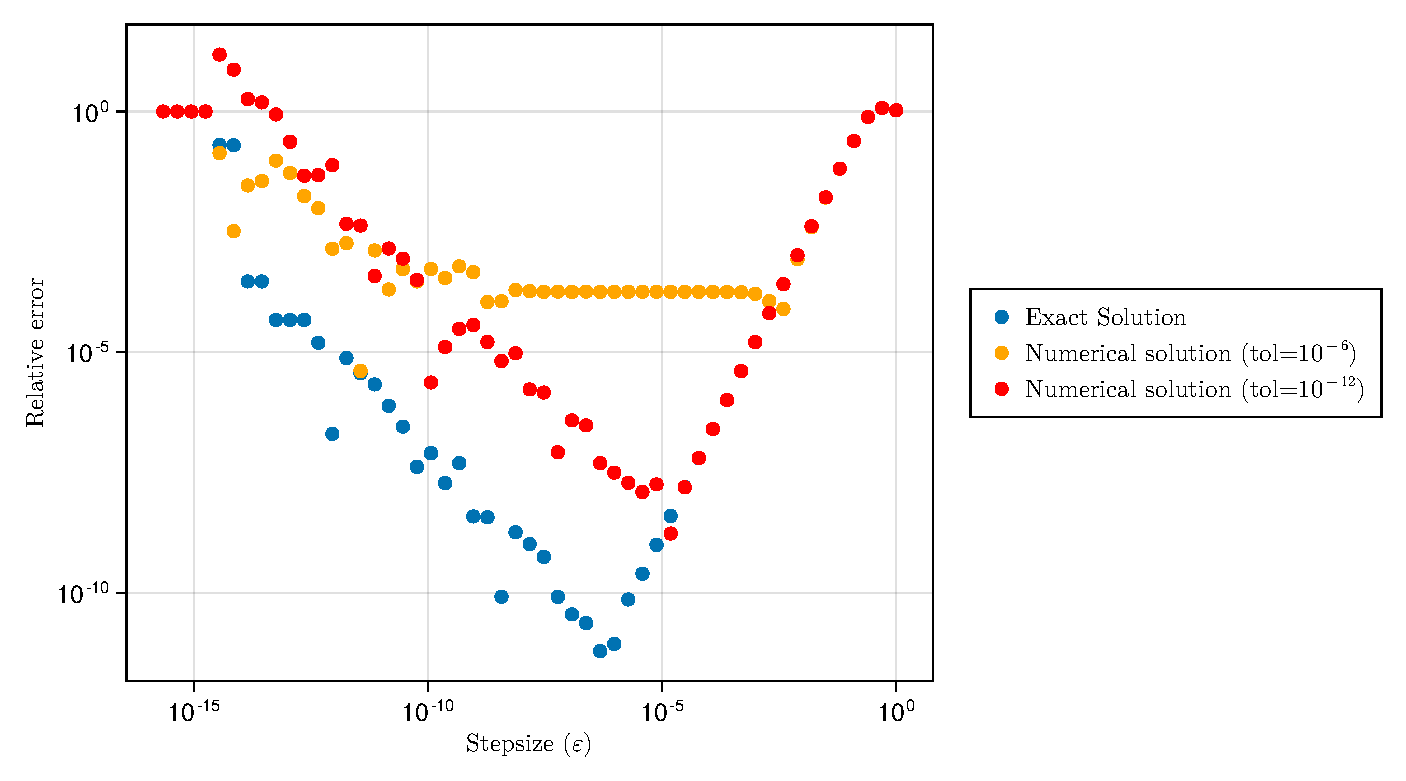
\includegraphics[width=0.85\textwidth]{../code/finite_differences/finite_difference_derivative.pdf}
    \caption{Absolute relative error when computing the gradient of the function $u(t) = \sin (\omega t)/\omega$ with respect to $\omega$ at $t=10.0$ as a function of the stepsize $\varepsilon$. Here $u(t)$ corresponds to the solution of the differential equation $u'' + \omega^2 u = 0$ with initial condition $u(0)=0$ and $u'(0)=1$. The blue dots correspond to the case where this is computed with finite differences. The red and orange lines are for the case where $u(t)$ is numerically computed using the default Tsitouras solver \cite{Tsitouras_2011} from \texttt{OrdinaryDiffEq.jl} using different tolerances. The error when using a numerical solver is larger and it is dependent on the numerical precision of the numerical solver. }
    \label{fig:finite-diff}
\end{figure}

Implementing forward AD using dual numbers is usually carried using \textit{operator overloading} \cite{Neuenhofen_2018}. 
This means expanding the object associated to a numerical value to include its dual components (derivative) and extending the definition of atomic algebraic functions. 
In Julia, this can be done by relying on multiple dispatch. 
The following example illustrates how to define a dual number and its associated binary addition and multiplication extensions. 
\begin{jllisting}
using Base: @kwdef

@kwdef struct DualNumber{F <: AbstractFloat}
    value::F
    derivative::F
end

# Binary sum
Base.:(+)(a::DualNumber, b::DualNumber) = DualNumber(value = a.value + b.value, derivative = a.derivative + b.derivative)

# Binary product 
Base.:(*)(a::DualNumber, b::DualNumber) = DualNumber(value = a.value * b.value, derivative = a.value*b.derivative + a.derivative*b.value)
\end{jllisting}
% and then we can simply evaluate derivatives by evaluating the derivative component of the dual number that results from the combination of operations
% \begin{jllisting}
% a = DualNumber(value=1.0, derivative=1.0)

% b = DualNumber(value=2.0, derivative=0.0)
% c = DualNumber(value=3.0, derivative=0.0)

% result = a * b * c
% println("The derivative of a*b*c with respect to a is: ", result.derivative)
% \end{jllisting}
% Notice that in this last example the dual numbers \texttt{b} and \texttt{c} were initialized with a derivative value equal to zero, while \texttt{a} with a value equal to one. 
% This is because we were interested in computing the derivative with respect to \texttt{a}, and then $\frac{\partial a}{\partial a} = 1$, while $\frac{\partial b}{\partial a} = \frac{\partial c}{\partial a} = 0$. 
We can also extend the definition of standard functions by simply applying the chain rule and storing the derivative in the dual variable following Equation \eqref{eq:dual-number-function}:
\begin{jllisting}
function Base.:(sin)(a::DualNumber)
    value = sin(a.value)
    derivative = a.derivative * cos(a.value)
    return DualNumber(value=value, derivative=derivative)
end
\end{jllisting}
% With all these pieces together, we are able to propagate forward the value of a single-valued derivative through a series of algebraic operations. 
In the Julia ecosystem, \texttt{ForwardDiff.jl} implements forward mode AD with multidimensional dual numbers \cite{RevelsLubinPapamarkou2016}. 
Notice that a major limitation of the dual number approach is that we need a dual variable for each variable we want to differentiate. 
Implementations of forward AD using dual numbers and computational graphs require a number of operations that increases with the number of variables to differentiate, since each computed quantity is accompanied by the corresponding gradient calculations \cite{Griewack-on-AD}. 
This consideration also applies to the other forward methods, including finite differences and complex-step differentiation, which makes forward models inefficient when differentiating with respect to many parameters. 


Notice that both AD based in dual number and complex-step differentiation introduce an abstract unit ($\epsilon$ and $i$, respectively) associated with the imaginary part of the extender value that carries forward the numerical value of the gradient.
% This resemblance between the methods makes them susceptible to the same advantages and disadvantages: easiness of implementation with operator overloading; and inefficient scaling with respect to the number of variables to differentiate. 
Although these methods seem similar, it is important to remark that AD gives the exact gradient, while complex step differentiation relies on numerical approximations that are valid just when the stepsize $\varepsilon$ is small. 
The next example shows how the calculation of the gradient of $\sin (x^2)$ is performed by these two methods:
\begin{equation}
\renewcommand{\arraystretch}{1.5}
\begin{tabular}{@{} l @{\qquad} l @{\qquad} l @{}}
Operation & AD with Dual Numbers  & Complex Step Differentiation \\
$x$ & $x + \epsilon$    & $x + i \varepsilon$ \\
$x^2$ & $x^2 + \epsilon \, (2x)$  & $x^2 - \varepsilon^2 + 2i\varepsilon x$\\
$\sin(x^2)$  & $\sin(x^2) + \epsilon \, \cos(x^2) (2x)$ &
$\sin(x^2 - \varepsilon^2) \cosh (2i\varepsilon) + i \, \cos(x^2 - \varepsilon^2) \sinh (2i\varepsilon)$
\end{tabular}
\label{eq:AD-complex-comparision}
\end{equation}
While the second component of the dual number has the exact derivative of $\sin(x^2)$, it is not until we take $\varepsilon \rightarrow 0$ than we obtain the derivative in the imaginary component for the complex step method
\begin{equation}
    \lim_{\varepsilon \rightarrow 0} \, \frac{1}{\varepsilon} \, \cos(x^2 - \varepsilon^2) \sinh (2i\varepsilon) 
    = 
    \, \cos(x^2) (2x).
\end{equation}
The stepsize dependence of the complex step differentiation method makes it resemble more to finite differences than AD with dual numbers. 
This difference between the methods also makes the complex step method sometimes more efficient than both finite differences and AD \cite{Lantoine_Russell_Dargent_2012}, an effect that can be counterbalanced by the number of extra unnecessary operations that complex arithmetic requires (see last column of \eqref{eq:AD-complex-comparision}) \cite{Martins_Sturdza_Alonso_2003_complex_differentiation}.
It is also important to remark that many modern software already have support for complex number arithmetic, making complex step differentiation very easy to implement.

\subsubsection{Backpropagation}

The libraries \texttt{ReverseDiff.jl} and \texttt{Zygote.jl} use callbacks to compute gradients. When gradients are being computed with less than $\sim 100$ parameters, the former is faster (see documentation).

\subsection{Solver-based methods}

Sensitivity methods based on numerical solvers tend to be better adapted to the structure and properties of the underlying ODE (stiffness, stability, accuracy) but also more difficult to implement.  
This difficulty arises from the fact that the sensitivity method needs to deal with some numerical and computational considerantions, including how to handle matrix/Jacobian-vector products; numerical stability of the forward/backward solver; and memory-time tradeoff. 
These factors are further exacerbated by the number of ODEs and parameters in the model. 
% While explicit methods can be preferable for non-stiff problems, Rosenblock methods can be 
Just a few modern scientific software have the capabilities of handling ODE solvers and computing their sensitivities at the same time. 
The include \texttt{CVODES} within \texttt{SUNDIALS} in C \cite{serban2005cvodes, SUNDIALS-hindmarsh2005sundials}; \texttt{ODESSA} \cite{ODESSA} and \texttt{FATODE} (discrete adjoints) \cite{FATODE2014} both in Fortram; \texttt{SciMLSensitivity.jl} in Julia \cite{rackauckas2020universal}; \texttt{Dolfin-adjoint} based on the \texttt{FEniCS} Project \cite{dolfin2013, dolfin2018}. 

It is important to remark that the underlying machinery of all solvers relies on solvers for linear systems of equations, which can be solved in dense, band (sparse), and Krylow mode. 
% This implies that methods based on numerical solvers are, in principle, more difficult to implement but also more efficient in computing gradients for complex differential equations. 
Another important consideration is that all these methods have subroutines to compute the VJPs involved in the sensitivity and adjoint equations. 
This calculation is carried out by another sensitivity method (finite differences, AD) and this also plays a central role at the moment of analyzing the accuracy and stability of the adjoint method. 

\subsubsection{Sensitivity equation}

\subsubsection{Solving the adjoint}

% Distinctio between discrete and continuous
% Discrete are the exact gradient of the computer program, continuous are not. 
% There is no flexibilty in discrete adjoitns, but there is in continuous
% Human effort required to compute discrete adjoints is large \cite{FATODE2014}

An equally important consideration when working with adjoints is when these are numerically stable. 
Some works have shown that continuous adjoints can lead to unstable sensitivities \cite{Jensen_Nakshatrala_Tortorelli_2014}.
Implicit forward schemes can give rise to explicit backwards schemes, leading to unstable solutions for the gradient. 

\vspace*{10px}
\noindent \textbf{\textit{Solving the backwards mode}}
\vspace*{5px}

The bottleneck of this method is the calculation of the adjoint since in order to solve the adjoint equation we need to know $u(t)$ at any given time. 
Effectively, notice that the adjoint equation involves the terms $f(u, \theta, t)$ and $\frac{\partial h}{\partial u}$ which are both functions of $u(t)$. 
There are different ways of addressing the evaluation of $u(t)$ during the backwards step.
\begin{enumerate}[label=(\roman*)]
    \item \textbf{Dense Store.} During the forward model, we can just store in memory all the intermediate states of the numerical solution. 
    This leads to heavy-memory expensive algorithms. 
    \item \textbf{Re-solve.} Solve again the original ODE together with the adjoint as the solution of the reversed augmented system \cite{chen_neural_2019}
    \begin{equation}
    \frac{d}{dt}
    \begin{bmatrix}
       u \\
       \lambda \\
       \frac{dL}{d\theta}
    \end{bmatrix}
    = 
    \begin{bmatrix}
       -f \\
       - \frac{\partial f}{\partial u}^T \lambda - \frac{\partial h}{\partial u}^T \\
       - \lambda^T \frac{\partial f}{\partial \theta} - \frac{\partial h}{\partial \theta}
    \end{bmatrix}
    % = 
    % - [ 1, \lambda^T, \lambda^T ]
    % \begin{bmatrix}
    %    f & \frac{\partial f}{\partial u} & \frac{\partial f}{\partial \theta} \\
    %    0 & 0 & 0 \\
    %    0 & 0 & 0
    % \end{bmatrix},
    \qquad 
    \begin{bmatrix}
       u \\
       \lambda \\
       \frac{dL}{d\theta}
    \end{bmatrix}(t_1)
    = 
    \begin{bmatrix}
       u(t_1) \\
       \frac{\partial L}{\partial u(t_1)} \\
       \lambda(t_0)^T s(t_0)
    \end{bmatrix}.
    \end{equation}
    However, computing the ODE backwards can be unstable and lead to large numerical errors \cite{kim_stiff_2021, Zhuang_2020}. 
    \item \textbf{Checkpointing. } Also known as windowing, checkpointing is a technique that trade-offs memory and time by saving intermediate states of the solution in the forward pass and recalculating the solution between intermediate states in the backwards mode \cite{Checkpoiting_2023, griewank2008evaluatingderivatives}. 
    This is implemented in \texttt{Checkpointing.jl} \cite{Checkpoiting_2023}.
\end{enumerate} 

One way of solving this system of equations that ensures stability is by using implicit methods. 
However, this requires cubic time in the total number of ordinary differential equations, leading to a total complexity of $\mathcal O((n+p)^3)$ for the adjoint method.
Two alternatives are proposed in \cite{kim_stiff_2021}, the first one called \textit{Quadrature Adjoint} produces a high order interpolation of the solution $u(t)$ as we move forward, then solve for $\lambda$ backwards using an implicit solver and finally integrating $\frac{dL}{d\theta}$ in a forward step.
This reduces the complexity to $\mathcal O (n^3 + p)$, where the cubic cost in the number of ODEs comes from the fact that we still need to solve the original stiff differential equation in the forward step. 
A second but similar approach is to use an implicit-explicit (IMEX) solver, where we use the implicit part for the original equation and the explicit for the adjoint. 
This method also will have complexity $\mathcal O (n^3 + p)$.

\vspace*{10px}
\noindent \textbf{\textit{Solving the quadrature}}
\vspace*{5px}

Another computational challenge in the computation of the continuous adjoint is how the integral in Equation \eqref{eq:casa-final-loss-gradient} is numerically evaluated. 
Some methods save computation by noticing that the last step in the continuous adjoint method of evaluating $\frac{dL}{d\theta}$ is an integral instead of an ODE, and then can be evaluated as such without the need to include it in the tolerance calculation inside the numerical solver \cite{that-is-not-an-ode}.

Numerical solutions of the integral 
\begin{equation}
    \int_{t_0}^{t_1} 
    \approx
    \sum 
\end{equation}
Gaussian quadrature is the faster method to evaluate one-dimensional integrals \cite{Norcliffe_gaussquadrature_2023}.

Weights and knots are obtained in order to maximize the order in which polynomials are exactly integrated \cite{stoer2002-numerical}. 

\subsubsection{Further considerations}

% In SUNDIALS, the VJPs involved in the sensitivity and adjoint method are handled using finite differences unless specified by the user \cite{SUNDIALS-hindmarsh2005sundials}.
% In FATODE, these can be computed with finite differences, AD or provides by the user.